%*******************************************************************************
%****************************** Third Chapter *********************************
%*******************************************************************************

\chapter{Proposed Methods}

\ifpdf
    \graphicspath{image/}
\fi


% \section{\label{sec:level1}Proposed Methods}

In this part, a new LSB replacement method named LSB-pair which is based on pair pixel matching is proposed. Some extension LSB-pair methods have been developed from this idea, extending its application range. In this part, all methods are designed to embed messages into grayscale image, where pixel values are stored as 8 bit unsigned integers. In order to differentiate the existing LSB replacement method and our modified LSB methods; we use \textit{original LSB replacement method} or \textit{regular LSB replacement method} to represent the \textit{existing LSB replacement method}; we use \textit{extension LSB-pair methods} to indicate our extension methods which based on LSB-pair method; we use \textit{the LSB-pair methods} to represent LSB-pair and its extension methods.


\section{\label{sec:level1}LSB-pair}

This function, named LSB-pair, tries to find pairs of pixels which would reduce watermarked image distortion from embedding. Before the start of pair detection, the carrier image should be transformed into a one-dimensional data. Figure 3.1 shows how to convert a picture, which is two-dimensional, into one dimension.

\begin{figure}[H]
 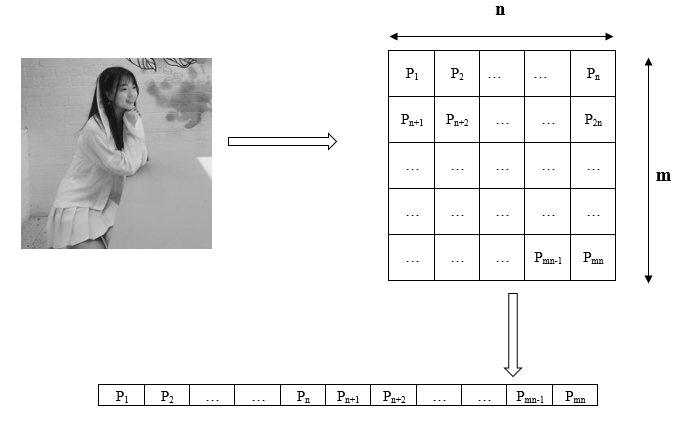
\includegraphics[width=\columnwidth]{image/Convert_image_as_one-dimension_matrix.png}
 \caption{Convert image as one-dimension matrix}
 \label{fig:figure}
\end{figure}

With one-dimension data structure, we can use an array list to denote any pixels in the carrier image. For instance, \(P_{i}\) represents a specific pixel in the carrier image, with \(i\) denoting its sequence number in the data. Symbol \(G(P_{i})\) means the value of gray level in pixel \(P_{i}\). The value of \(G(P_{i})\) is an integer which ranges from 0 to 255. When converting watermarked message into binary, we can use \(M_{i}\) to present the \(i^{th}\) binary value of this watermarking message. Hence, the value of \(M_{i}\) is either 0 or 1. \(M_{i}\) and \(M_{i+1}\) are corresponding message bits respectively for \(P_{i} \text{ and } P_{i+1}\). Finally, the notation \(LSB(G(P_{i}))\) represents the last bit of gray level value on this pixel. For example, if the gray level of the \(28^{th}\) pixel was 125, we could use math formula \(LSB(G(P_{28})) = 1\) to present the LSB of \(28^{th}\) pixel. If the gray level of the \(29^{th}\) pixel was 126, we had \(LSB(G(P_{29}))\) is 0, etc. 

Based on the definition above, two adjacent pixels \(P_{i}\) and \(P_{i+1}\) are regarded as a LSB-pair pixels if they satisfy the conditions (3.1) and (3.2): 

\begin{equation}
\\ G(P_{i}) = G(P_{i+1}) + 1 \quad \text{ or } \quad G(P_{i}) = G(P_{i+1}) - 1
\end{equation}
\begin{equation}
LSB(G(P_{i})) \neq M_{i} \quad \text{ and } \quad LSB(G(P_{i+1})) \neq M_{i+1}
\end{equation}

We can use one sentence to conclude this definition: \textit{two adjacent pixels with adjacent gray levels and their LSB are different from corresponding message bits}.

After obtaining our LSB pairs, the next step is to find out how the distortion changes when embedding the message. Due to the fact that each pixel in grayscale image occupies 8 bits, we can use a list of 256 ordered elements to represent the image energy distribution or we can call it distortion directly. Each element means the frequency of a specific gray level. The distortion list may be written as:
\[D = (d_{0}, d_{1}, d_{2} … , d_{253}, d_{254}, d_{255})\]
For example, \(d_{35} = 47\) represents the total number of gray level 35 is 47. In order to calculate the distortion changes after watermarking, the original image distortion \(d_{1}\) and the watermarked image distortion \(d_{2}\) are required. The difference between \(d_{1}\) and \(d_{2}\): \(D’ = d_{2} - d_{1}\) is the distortion change which will be used in the latter evaluation. In this case: \(D’ = (d’_{0}, d’_{1}, d’_{2}…, d’_{253}, d’_{254}, d’_{255})\), \(d’35 = 47\) means the frequency of gray level 35 in watermarked image is 47 greater than original image. Therefore, if no message is embedded, all elements in \(D’\) should be 0.


There are two different situations when using LSB-pair method to embed messages. Firstly, suppose there are two pixels: \(G(P_{i}) = 124\), \(G(P_{i+1}) = 125\) and message bits: \(M_{i} = 1\), \(M_{i+1} = 0\). The LSB value of these two pixels can be obtained from calculation: \(LSB(G(P_{i})) = 0\), \(LSB(G(P_{i+1})) = 1\). Because these pixels meet the requirements (3.1) and (3.2), they are regarded as a pair. Assuming the distortion change before doing LSB replacement is:
\[D’_{before} = (…, d_{124} = a, d_{125} = b, …)\]
Then embed the $i^{\text{th}}$ message bit into this image, we have new \(G'(P_{i})\) and \(D’_{after}\): 
\[G’(P_{i}) = 125\]
\[D’_{after} = (…, d_{124} = a - 1, d_{125} = b + 1, …)\]

Then embed the $(i+1)^{\text{th}}$ message bit into this image, we have new \(G’(P_{i+1})\) and \(D’_{after}\): 
\[G’(P_{i+1}) = 124\]
\begin{align*} 
D’_{after}  &= (…, d_{124} = a - 1 + 1, d_{125} = b + 1 - 1, …)\\
            &= (…, d_{124} = a, d_{125} = b, …)\\
            &= D’_{before}
\end{align*}
\[ \Rightarrow D’_{after} - D’_{before} = 0\]
In this situation, distortion difference equals to 0 means that the distortion is not changed after embedding watermarking messages.

Another situation is that when \(G(P_{i}) = 125\), \(G(P_{i+1}) = 126\), \(M_{i} = 0\), \(M_{i+1} = 1\). Assume the distortion change before watermarking is \(D’_{before} = (…, d_{124} = a, d_{125} = b, d_{126} = c, d_{127} = d, …)\). Then using LSB replacement method to embed message, we have: 
\[G’(P_{i}) = 124\] 
\[G’(P_{i+1}) = 127\]
\[D’_{after} = (…, d_{124} = a + 1, d_{125} = b - 1, d_{126} = c - 1, d_{127} = d + 1, …)\]


After that, calculating the distortion difference: 
\[D’_{after} - D’_{before} = (|a + 1| - |a|) + (|b - 1| - |b|) + (|c - 1| - |c|) + (|d + 1| - |d|)\]

According to the definition, \(D’_{after} - D’_{before} < 0\) means that after embedding message, the distortion of the image is reduced and vice versa. Assume \(a > 0, b < 0, c < 0 \quad and \quad d > 0\), then we have:

\begin{align*} 
D’_{after} - D’_{before}    &= & & (|a + 1| - |a|) + (|b - 1| - |b|)\\
                            &  & & + (|c - 1| - |c|) + (|d + 1| - |d|)\\
                            &= & & (a + 1 - a) + (1 - b + b) \\
                            &  & & + (1 - c + c) + (d + 1 - d)\\
                            &= & & 1 + 1+ 1+ 1\\
                            &= & & 4 > 0
\end{align*}

However, when \(a + 1 < 0, b - 1 > 0, c - 1 > 0 \quad and \quad d + 1 < 0\)
\begin{align*} 
D'_{after} - D'_{before}    &= & & (|a + 1| - |a|) + (|b - 1| - |b|)\\
                            &  & & +(|c - 1| - |c|) + (|d + 1| - |d|)\\
                            &= & & ( - 1 - a + a) + (b - 1 - b)\\
                            &  & & + (c - 1 - c) + ( - 1 - d + d)\\
                            &= & & - 1 - 1 - 1 - 1\\
                            &= & & -4 < 0
\end{align*}
Besides these two specific situations, there are various permutations and combinations of the value of a, b, c and d. However, in LSB-pair methods, we are only interested in whether if the value of $D’_{after} - D’_{before}$ is positive or negative.  In other words, in this method there are only two interesting situations: increasing change in distortion or decreasing change. Additionally, the distortion change can be 0 in some situations; in order to reduce the algorithm complexity, we regard the distortion as not changing and distortion increasing as the same class.

In the situation of \(G(P_{i}) = 124\), \(G(P_{i+1}) = 125\), the distortion is not changed. Because after embedding, we have: \(G’(P_{i}) = 125, G’(P_{i+1}) = 124\), the total number of gray level 124 and 125 does not change. It looks like these two pixels swap their position (values). It inspires a solution to handle the second situation. Since \(G(P_{i}) = 125, G(P_{i+1}) = 126, M_{i} = 0, M_{i+1} = 1\), if swap the position of two pixels before embedding, the result will be: \(G’(P_{i}) = 126, G’(P_{i+1}) = 125\). Then, using LSB replacement method, it is obvious that the distortion would not change after embedding. However, when applying regular LSB replacement for the second situation directly, the distortion change can be both positive and negative. Hence, the idea of LSB-pair is swapping pixels before using LSB replacement when the distortion change is positive and using regular LSB replacement when distortion change is negative. One thing we need to clear is that the distortion \(D'\) will not change after swapping two pair pixels because the gray level distribution is not changing.

An example to outline how this method works can be found in the FIG 3.2; if there are two pixels, \(G(P_{i}) = 125, G(P_{i+1}) = 126\), we apply LSB replacement at first, then compare the distortion change. Depending on whether it is positive or negative, we can choose between swapping pixels values before using LSB replacement or to use regular LSB replacement directly. 


One more thing we need to pay attention to is that just swapping pixels value is the same as swapping pixels value when using LSB replacement. This conclusion is not hard to prove. From the LSB pair definition, there have two main classes: \circled{1} \(G(P_{i}) = G(P_{i+1}) + 1\) \textit{or} \circled{2} \(G(P_{i}) = G(P_{i+1}) - 1\) . After swapping pixels value, we have \circled{1} \(G(P’_{i}) = G(P_{i}) - 1, G(P’_{i+1}) = G(P_{i+1}) + 1\) \textit{and} \circled{2} \(G(P’_{i}) = G(P_{i}) + 1, G(P’_{i+1}) = G(P_{i+1}) - 1\) which correspond respectively. Then moving to their corresponding message bits: \(LSB(G(P_{i})) \neq M_{i}\) \textit{and} \(LSB(G(P_{i+1})) \neq M_{i+1}\), it is not hard to get that \(LSB(G(P’_{i})) = M_{i}\) \textit{and} \(LSB(G(P’_{i+1})) = M_{i+1}\). The pixels value will not change after applying LSB replacement method, because the last bit of each pixel is the same as its corresponding message bit. With this knowledge, we can reduce the LSB-pair algorithm complexity by simplifying swapping pixels value and apply LSB replacement to swapping pixels value only. 


\begin{figure}[h]
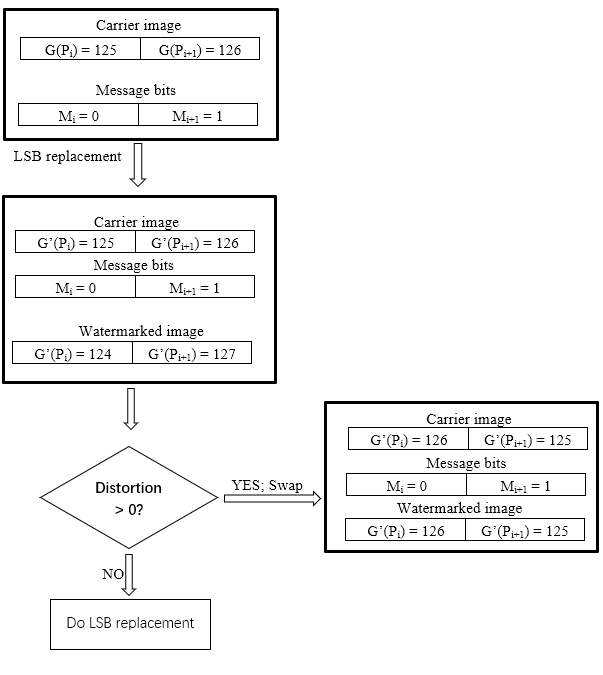
\includegraphics[width=\columnwidth]{image/LSB-pair_example.PNG}
\caption{LSB-pair embedding}
\label{fig:figure}
\end{figure}


In summary, this methods checks each pixel to find out pixel pair which satisfies requirements (3.1) and (3.2). Then we check the distortion change (difference) \(D'_{after} - D'_{before}\); if distortion change is larger than 0, swap two pixels' position. Otherwise, we apply the original LSB replacement method. It can be concluded by following steps (FIG 3.3):
\begin{enumerate}
\item Check current pixel \(P_{i}\) and next pixel \(P_{i+1}\) is a pair or not. If not, go to step (5), otherwise, go to step (2).
\item Calculate the distortion change \(D'_{after} - D_{before}\) for regular LSB replacement, if it larger than 0, go to step (3), otherwise, go to step (4)
\item Swap two pixels position (value), then jump next iteration, go to one after next iteration.
\item Do LSB replacement for this pixel \(P_{i}\) and next pixel \(P_{i+1}\), then jump next iteration, go to one after next iteration.
\item Do LSB replacement for current pixel \(P_{i}\) then go to next iteration for next pixel.
\end{enumerate}




\begin{figure}[h]
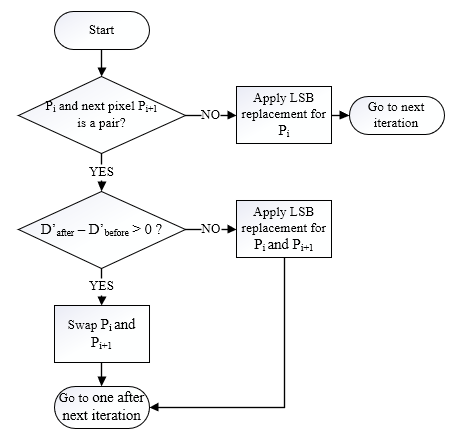
\includegraphics[width=\columnwidth]{image/processing_map.PNG}
\caption{LSB-pair processing map}
\label{fig:figure}
\end{figure}


\section{\label{sec:level1}LSB-triple-pair}

From our experiment for LSB-pair, we found that 0.47\% of pixels meet the requirements (3.1) and (3.2), and 0.25\% of the pixels are in position for swapping to reduce the image distortion. The experiment results show that LSB-pair is rare to find and have very limited performance on reducing watermarked image distortion. With this concern, there is a demand to expand LSB-pair method the range of application. Our modified method called LSB-triple-pair, it changes the requirements of the LSB-pair to expand the range of application.

The LSB-triple-pair method is a modification of LSB-pair which uses three pixels to find a pair. In the previous method, each logic iteration considers two adjacent pixels \(P_{i}\) and \(P_{i+1}\) and their corresponding message bits \(M_{i}\) and \(M_{i+1}\). In this method, three pixels are considered in each iteration: \(P_{i}, P_{i+1} and P_{i+2}\). The idea is, when the first and second pixel do not meet the condition (3.1) and (3.2) or distortion reduce requirements, this algorithm will try to find a pair between the first and third pixel to reduce the image distortion. The processing steps are:

\begin{enumerate}
\item Check current pixel \(P_{i}\) and next pixel \(P_{i+1}\) is a pair or not. If not, go to step (5), otherwise, go to step (2).
\item Calculate the distortion change for regular LSB replacement \(D'_{after} - D_{before}\), if it is \textbf{greater than or equal to} 0, go to step (4), otherwise, go to step (3).
\item Do LSB replacement for this pixel \(P_{i}\) and next pixel \(P_{i+1}\), then go one after next iteration.
\item Check current pixel \(P_{i}\) and the one after next pixel \(P_{i+2}\) is a pair or not. If not, go to step (5), otherwise, go to step (6).
\item Do LSB replacement for pixel \(P_{i}\), \(P_{i+1}\), \(P_{i+2}\) than jump two iterations, go to the fourth iteration.
\item Calculate the distortion change for apply LSB replacement on these three pixels \((D’_{after} - D’_{before})\), if it lager than 0, go to step (7), otherwise, go to step (5).
\item Swap the first and the third pixels position (value), do LSB replacement on the second pixel then jump next two iterations, go to the fourth iteration.
\end{enumerate}

For instance, there are three continuous pixels: \(G(P_{i}) = 125, G(P_{i+1}) = 124, G(P_{i+2}) = 126\), and their corresponding message bits: \(M_{i} = 0, M_{i+1} = 1 M_{i+2} = 1\). In this situation, first two pixels \(P_{i}\) and \(P_{i+1}\) meet the requirements (3.1) and (3.2). However, from the distortion definition, the distortion will not change after applying LSB replacement. Therefore, according to the algorithm, the value of these two pixels will not swap then the process will compare the first pixel with the third pixel. It is clear that \(P_{i}\) and \(P_{i+2}\) meet the requirements (3.1) and (3.2), assuming the distortion change will be greater than 0 after applying regular LSB replacement method, this method will swap \(P_{i}\) and \(P_{i+2}\) value then apply LSB replacement to these three pixels. FIG 3.4 shows the processing map.


\begin{figure}[h]
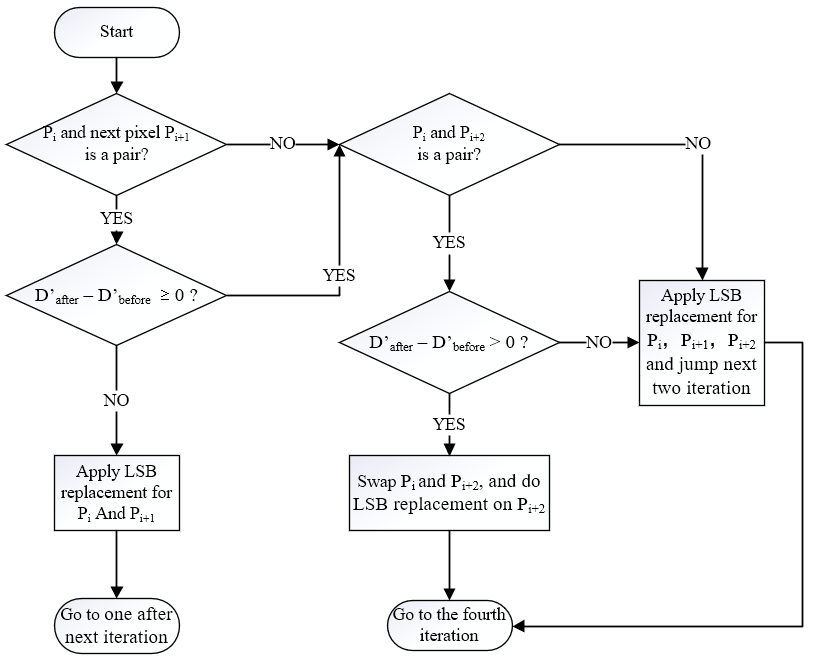
\includegraphics[width=\columnwidth]{image/processing_map_triple.PNG}
\caption{LSB-triple-pair processing map}
\label{fig:figure}
\end{figure}    




\section{\label{sec:level1}LSB-crossLine-pair}

LSB-crossline-pair is another method which extends from LSB-pair. This method tries to find the pixel pairs of current pixel with next line pixel in the carrier image. In this algorithm, we need to change image sequencing from one dimension back to two dimensions. FIG 3.5 shows how this method finds pixel pairs with next line pixel. For example, if the carrier image has \(n\) pixels in horizontal and \(m\) pixels in vertical, this algorithm will try to find a pair between pixel \(P_{i}\) and \(P_{i+n}\). The motivation of this method is also to extend the application range of LSB-pair.  

In this case, in order to avoid embedding system crush, the algorithm will stop LSB-crossline-pair detecting and do LSB-pair detect only when moving to pixel which is in the last row. Another thing that we need to pay attention to is the possibility of jumping to specific iterations. Because the embedding algorithm is from one pixel to next pixel sequentially, for LSB-pair, when a crossline pair is detected, the algorithm would apply original LSB-pair or swap pixels value, then jump two adjacent iterations. However, in LSB-crossline-pair, it cannot jump to the iteration of the next line’s pixel immediately. In code level, it needs an extra list to record the \(P_{i+n}\), if \(P_{i}\) and \(P_{i+n}\) meet all requirements of swapping value. Before each iteration, the code will check this list to see whether we need to jump this iteration or not. However, in fact, this special situation cannot influence the result of LSB-crossline-pair detect. Because if \(P_{i}\) and \(P_{i+n}\) meet the conditions of value swap, the new \(P_{i+n}\) (previous \(P_{i}\)) cannot satisfy requirement (3.2), which is \(LSB(G(P_{i+n})) \neq M_{i+n}\). In our experiments and coding, we skip this swapped pixel checking function, in order to save CPU processing power and memory usage. Furthermore, logically, this makes no sense to check LSB-pair condition for an already swapped value pixel. This can be an optimisation for improving time-consuming and reducing algorithm complexity for LSB-crossline-pair method.  

The processing steps for LSB-crossline-pair are:

\begin{enumerate}
\item Check current pixel \(P_{i}\) is in the jump list or not. If yes, go to next iteration, otherwise, go to step (2).
\item Check current pixel \(P_{i}\) and next pixel \(P_{i+1}\) is a pair or not. If not, go to step (5), otherwise, go to step (3).
\item Calculate the distortion change for using regular LSB replacement \((D’_{after} - D’_{before})\), if it \textbf{greater than or equal to} 0, go to step (5), otherwise, go to step (4)
\item Do LSB replacement for this pixel \(P_{i}\) and next pixel \(P_{i+1}\), then jump next iteration, go to the one after iteration.
\item Check current pixel \(P_{i}\) and the one after next pixel \(P_{i+n}\) is a pair or not. If not, go to step (6), otherwise, go to step (7).
\item Do LSB replacement for pixel \(P_{i}, P_{i+1}, P_{i+n}\) , record \(P_{i+n}\) into jump list then jump next iterations, go to the third iteration.
\item Calculate the distortion change for applying LSB replacement on \(P_{i}\) and \(P_{i+n}\):  \((D’_{after} - D’_{before})\), if it greater than 0, go to step (8), otherwise, go to step (6).
\item Swap \(P_{i}\), and the \(P_{i+n}\) position (value), do LSB replacement on \(P_{i+1}\) then record \(P_{i+n}\) into jump list, after that, jump next iteration, go to the third iteration.
\end{enumerate}

For instance, there are three pixels: \(G(P_{i}) = 125, G(P_{i+1}) = 124, G(P_{i+n}) = 126\), and their corresponding message bits: \(M_{i} = 0, M_{i+1} = 1 M_{i+n} = 1\). In this situation, first two pixels \(P_{i}\) and \(P_{i+1}\) meet the requirements (3.1) and (3.2). However, from the distortion definition, the distortion will not change after applying LSB replacement. Therefore, according to the algorithm, the value of these two pixels will not swap then the process will compare the first pixel \(P_{i}\) with the next line pixel \(P_{i+n}\). It is clear that \(P_{i}\) and \(P_{i+n}\) meet the requirements (3.1) and (3.2), assuming the distortion change will be greater than 0 after applying regular LSB replacement method, this method will swap \(P_{i}\) and \(P_{i+n}\) value then record \(P_{i+n}\) to jump list. After that, apply LSB replacement to these three pixels.

\begin{figure}[h]
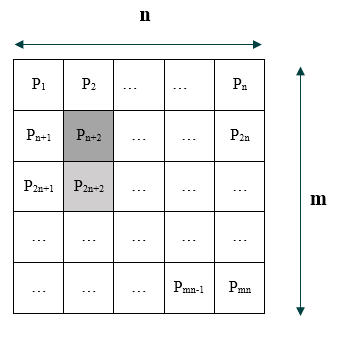
\includegraphics[width=\columnwidth]{image/LSB-crossline-pair.PNG}
\caption{LSB-crossline-pair}
\label{fig:figure}
\end{figure}   




\section{\label{sec:level1}Combination}

This extension method is called LSB-combination-pair; it aims to explore whether the combination of multiple LSB-pair methods can increase the performance of distortion reduction. The series of LSB-pair methods used in this section are LSB-pair, LSB-crossline-pair and LSB-triple-pair. As we have discussed above, all these methods can improve the performance of reducing watermarked image distortion. Therefore, it is possible that combining these three methods into one should have better performance than original LSB replacement as well as any of these three. 

As for the priority of pair finding in LSB-combine-pair. By comparing the performance of LSB-crossline-pair and LSB-triple-pair, the result shows that LSB-crossline-pair have better performance and more consistent in reducing image distortion than LSB-triple-pair. A detailed discussion and analysis of experiment result will be provided in next chapter. Hence, the idea of the new approach is to use LSB pair method at first; if these pixels are not a pair, try to find LSB-crossline-pair. If these pixels still do not meet the requirements of distortion reducing, then try to find a pair using LSB-triple-pair. FIG 3.6 shows a simplification processing map.


\begin{figure}[h]
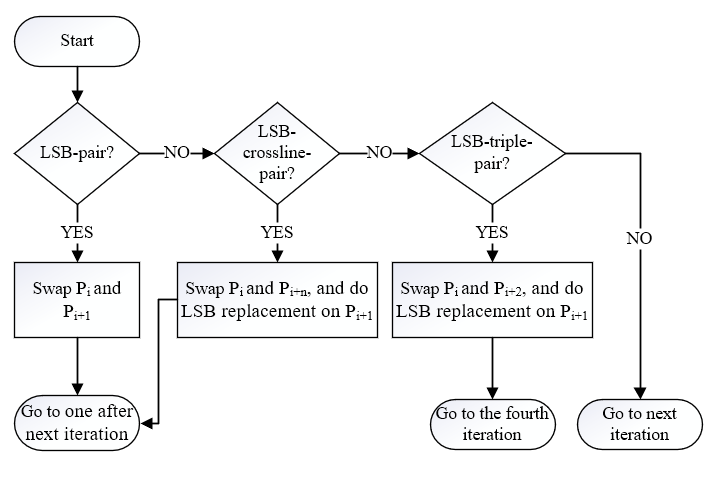
\includegraphics[width=\columnwidth]{image/processing_map_ultra.PNG}
\caption{LSB-combine-pair processing map}
\label{fig:figure}
\end{figure}  